\documentclass[a4paper, 11pt]{article}
\usepackage{comment} % enables the use of multi-line comments (\ifx \fi) 
\usepackage{fullpage} % changes the margin
\usepackage{enumitem}
\usepackage[T1]{fontenc}
\usepackage[polish]{babel}
\usepackage[utf8]{inputenc}
\usepackage{ragged2e}
\usepackage{graphicx}
\usepackage{datatool}
\usepackage{rotating}
\usepackage{placeins}
\usepackage{pdflscape}
\usepackage{float}
\usepackage{listings}
\usepackage{pdfpages}
\usepackage{xcolor} % for setting colors

\usepackage{color}

\usepackage{hyperref}
\hypersetup{
colorlinks,
citecolor=black,
filecolor=black,
linkcolor=black,
urlcolor=black
}


\lstset{frame=tb,
language=java,
aboveskip=3mm,
belowskip=3mm,
showstringspaces=false,
columns=flexible,
basicstyle={\small\ttfamily},
numbers=none,
numberstyle=\tiny\color{gray},
keywordstyle=\color[HTML]{EA1212},
commentstyle=\color{dkgreen},
stringstyle=\color{blue},
breaklines=true,
breakatwhitespace=true,
tabsize=3,
otherkeywords={},
morekeywords={}
}

\definecolor{dkgreen}{rgb}{0,0.6,0}
\definecolor{gray}{rgb}{0.5,0.5,0.5}
\definecolor{mauve}{rgb}{0.58,0,0.82}


\title{Raport z wykonania ćwiczenia Hibernate}
\author{Jakub Płotnikowski}
\date{Listopad 2019r.}


\begin{document}

    \maketitle
    \tableofcontents

    \newpage

    \section{III. Modyfikacja modelu - wprowadzenie Dostawcy (dokończenie z zajęć)}

    \subsection{Moment dodawania produktu}

    \begin{center}
        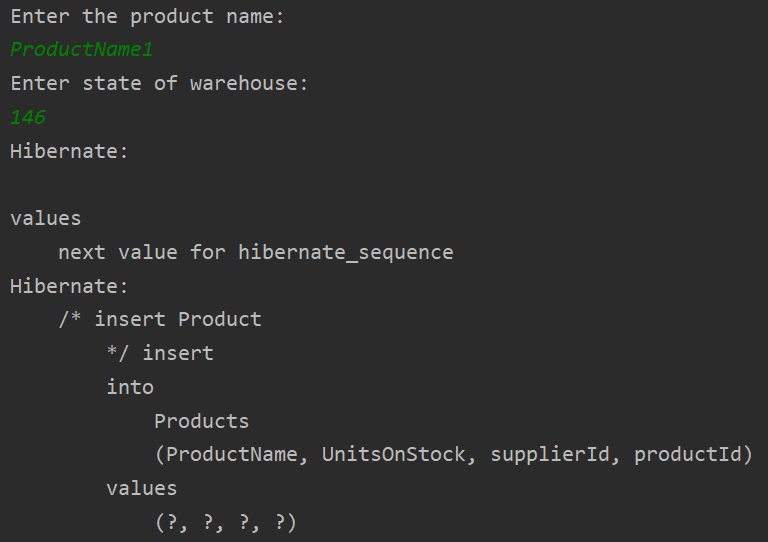
\includegraphics{images/point3/addProduct.png}
    \end{center}

    \subsection{Moment dodawania dostawcy}

    \begin{center}
        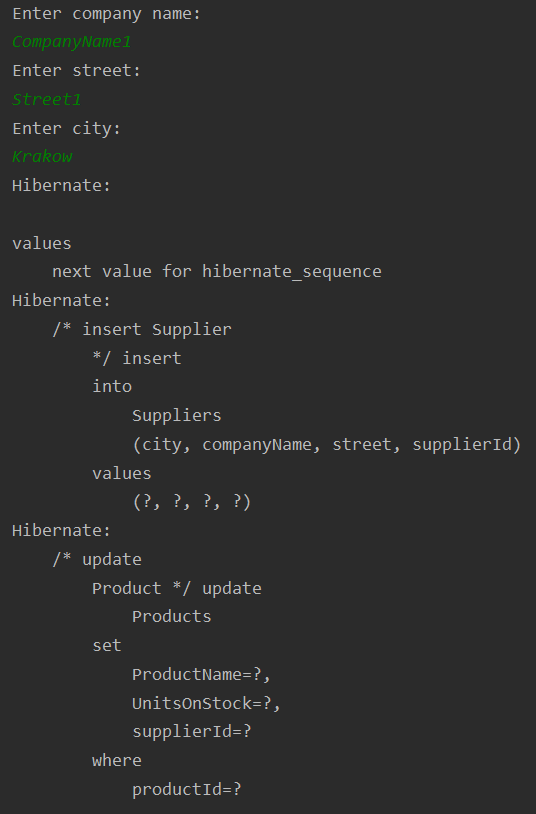
\includegraphics{images/point3/addSupplier.png}
    \end{center}

    \newpage

    \subsection{Kod klasy Product}
    \lstinputlisting[firstline=2]{source_code_and_ddl/point3/Product.java}

    \newpage

    \subsection{Kod klasy Supplier}
    \lstinputlisting[firstline=2]{source_code_and_ddl/point3/Supplier.java}

    \newpage



    \section{IVa. Odwrócenie relacji - wykorzystanie tabeli łącznikowej}

    \subsection{Pobranie informacji o dostawcy i produktach oraz dodanie ich do bazy}
    \begin{center}
        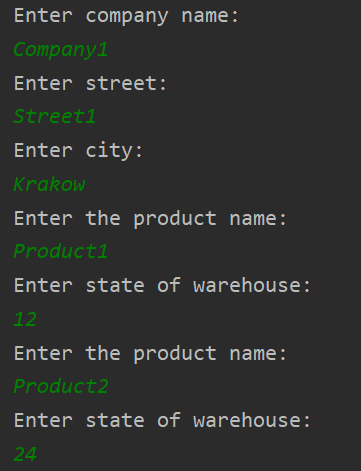
\includegraphics[scale=1.3]{images/point4_additional_table/addSupplierAndProducts.png}
    \end{center}

    \subsection{Zapytania wykonane przez Hibernate}
    \begin{center}
        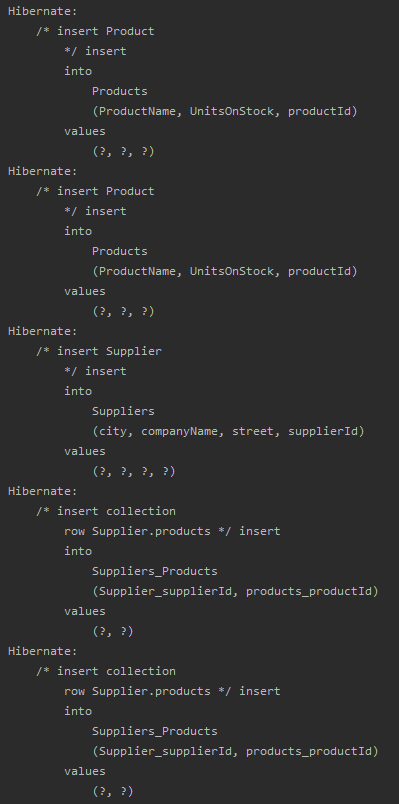
\includegraphics[scale=1.3]{images/point4_additional_table/hibernateQueries.png}
    \end{center}

    \newpage

    \subsection{Kod klasy Product}
    \lstinputlisting[firstline=2]{source_code_and_ddl/point4_additional_table/Product.java}

    \newpage

    \subsection{Kod klasy Supplier}
    \lstinputlisting[firstline=2]{source_code_and_ddl/point4_additional_table/Supplier.java}

    \newpage

    \subsection{Wyniki SELECT * z poszczególnych tabel}
    \subsubsection{Tabela Suppliers}
    \begin{center}
        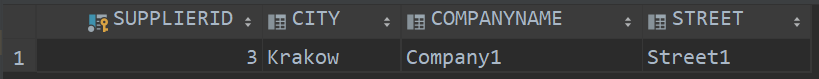
\includegraphics{images/point4_additional_table/SelectSuppliers.png}
    \end{center}

    \subsubsection{Tabela Products}
    \begin{center}
        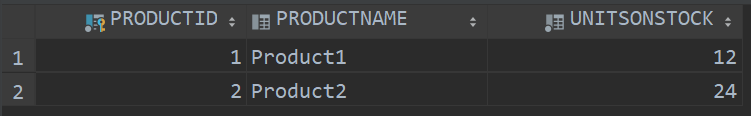
\includegraphics{images/point4_additional_table/SelectProducts.png}
    \end{center}

    \subsubsection{Tabela łącznikowa}
    \begin{center}
        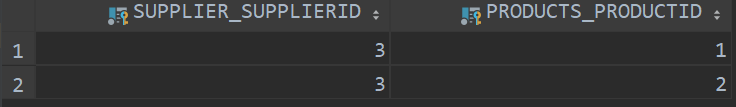
\includegraphics{images/point4_additional_table/SelectJoinTable.png}
    \end{center}

    \newpage

    \subsection{Kod DDL}
    \lstinputlisting{source_code_and_ddl/point4_additional_table/DDL.sql}

    \newpage



    \section{IVb. Odwrócenie relacji - brak tabeli łącznikowej}

    \subsection{Pobranie informacji o dostawcy i produktach oraz dodanie ich do bazy}
    \begin{center}
        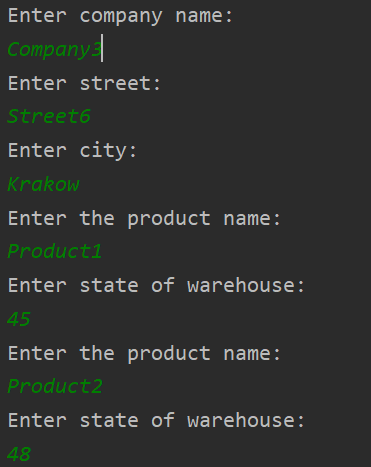
\includegraphics[scale=1.3]{images/point4_without_additional_table/addSupplierAndProducts.png}
    \end{center}

    \subsection{Zapytania wykonane przez Hibernate}
    \begin{center}
        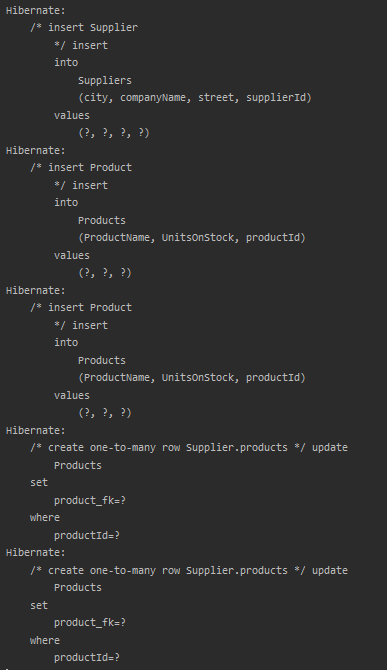
\includegraphics[scale=1.3]{images/point4_without_additional_table/hibernateQueries.png}
    \end{center}

    \newpage

    \subsection{Kod klasy Product}
    \lstinputlisting[firstline=2]{source_code_and_ddl/point4_without_additional_table/Product.java}

    \newpage

    \subsection{Kod klasy Supplier}
    \lstinputlisting[firstline=2]{source_code_and_ddl/point4_without_additional_table/Supplier.java}

    \newpage

    \subsection{Wyniki SELECT * z poszczególnych tabel}
    \subsubsection{Tabela Suppliers}
    \begin{center}
        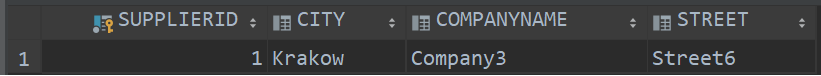
\includegraphics{images/point4_without_additional_table/SelectSuppliers.png}
    \end{center}

    \subsubsection{Tabela Products}
    \begin{center}
        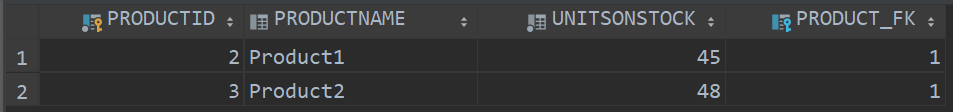
\includegraphics[scale=0.9]{images/point4_without_additional_table/SelectProducts.png}
    \end{center}

    \newpage

    \subsection{Kod DDL}
    \lstinputlisting{source_code_and_ddl/point4_without_additional_table/DDL.sql}

    \newpage



    \section{V. Relacja dwustronna. Dostawca - producent}

    \subsection{Pobranie informacji o dostawcy i produktach oraz dodanie ich do bazy}
    \begin{center}
        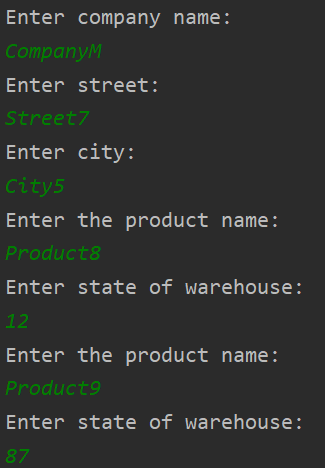
\includegraphics[scale=1.3]{images/point5/addSupplierAndProducts.png}
    \end{center}

    \subsection{Zapytania wykonane przez Hibernate}
    \begin{center}
        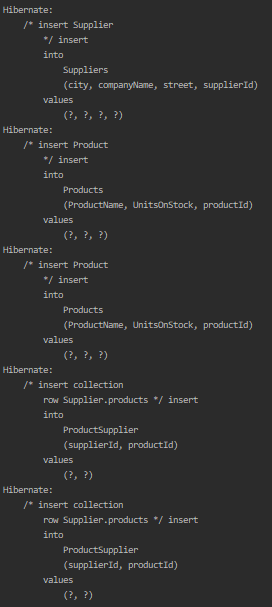
\includegraphics[scale=1.3]{images/point5/hibernateQueries.png}
    \end{center}

    \newpage

    \subsection{Kod klasy Product}
    \lstinputlisting[firstline=2]{source_code_and_ddl/point5/Product.java}

    \newpage

    \subsection{Kod klasy Supplier}
    \lstinputlisting[firstline=2]{source_code_and_ddl/point5/Supplier.java}

    \newpage

    \subsection{Wyniki SELECT * z poszczególnych tabel}
    \subsubsection{Tabela Suppliers}
    \begin{center}
        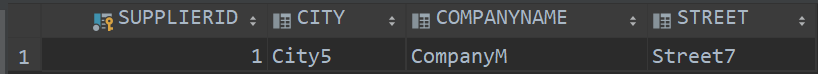
\includegraphics{images/point5/SelectSuppliers.png}
    \end{center}

    \subsubsection{Tabela Products}
    \begin{center}
        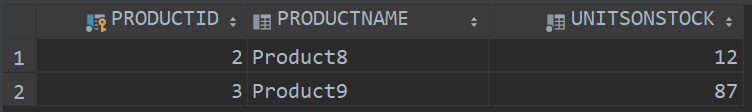
\includegraphics[scale=0.9]{images/point5/SelectProducts.png}
    \end{center}

    \subsubsection{Tabela łącznikowa}
    \begin{center}
        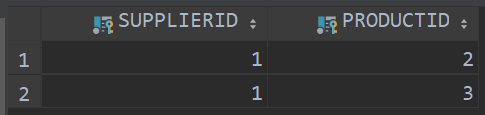
\includegraphics{images/point5/SelectJoinTable.png}
    \end{center}

    \newpage

    \subsection{Kod DDL}
    \lstinputlisting{source_code_and_ddl/point5/DDL.sql}

    \newpage



    \section{VI. Obsługa klasy Category}

    \subsection{Pobranie informacji o dostawcy, produkcie i kategorii}
    \begin{center}
        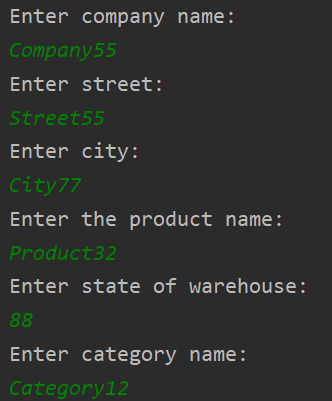
\includegraphics[scale=1.3]{images/point6/addSupplierProductAndCategory.png}
    \end{center}

    \subsection{Zapytania wykonane przez Hibernate}
    \begin{center}
        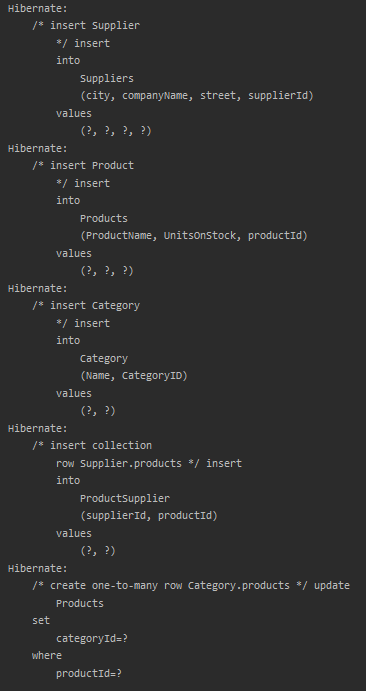
\includegraphics[scale=1.3]{images/point6/hibernateQueries.png}
    \end{center}

    \newpage

    \subsection{Kod klasy Product}
    \lstinputlisting[firstline=2]{source_code_and_ddl/point6/Product.java}

    \newpage

    \subsection{Kod klasy Supplier}
    \lstinputlisting[firstline=2]{source_code_and_ddl/point6/Supplier.java}

    \newpage

    \subsection{Kod klasy Category}
    \lstinputlisting[firstline=2]{source_code_and_ddl/point6/Category.java}

    \newpage

    \subsection{Wyniki SELECT * z poszczególnych tabel}
    \subsubsection{Tabela Suppliers}
    \begin{center}
        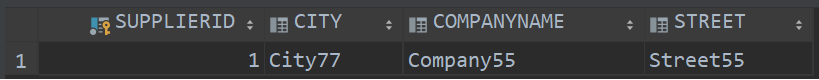
\includegraphics{images/point6/SelectSuppliers.png}
    \end{center}

    \subsubsection{Tabela Products}
    \begin{center}
        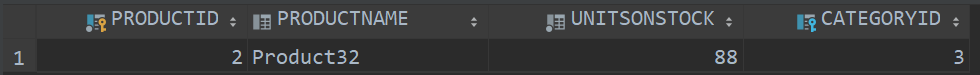
\includegraphics[scale=0.85]{images/point6/SelectProducts.png}
    \end{center}

    \subsubsection{Tabela ProductsSupplier}
    \begin{center}
        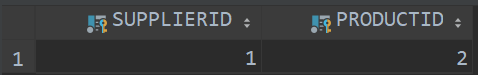
\includegraphics{images/point6/SelectProductsSupplier.png}
    \end{center}

    \subsubsection{Tabela Category}
    \begin{center}
        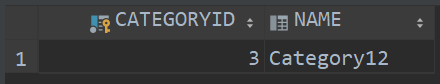
\includegraphics{images/point6/SelectCategories.png}
    \end{center}

    \newpage

    \subsection{Kod DDL}
    \lstinputlisting{source_code_and_ddl/point6/DDL.sql}

    \newpage



    \section{VII. Relacja wiele do wielu. Invoice - Product}

    \subsection{Pobranie informacji o firmie, produkcie i fakturze}
    \begin{center}
        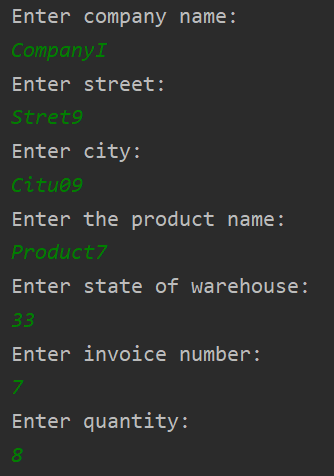
\includegraphics[scale=1.3]{images/point7/addCompanyProductInvoice.png}
    \end{center}

    \subsection{Zapytania wykonane przez Hibernate}
    \begin{center}
        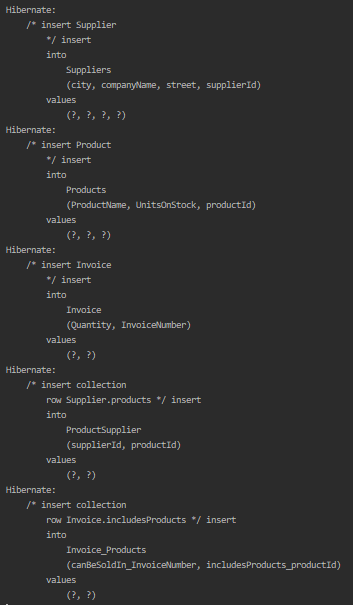
\includegraphics[scale=1.3]{images/point7/hibernateQueries.png}
    \end{center}

    \newpage

    \subsection{Kod klasy Product}
    \lstinputlisting[firstline=2]{source_code_and_ddl/point7/Product.java}

    \newpage

    \subsection{Kod klasy Supplier}
    \lstinputlisting[firstline=2]{source_code_and_ddl/point7/Supplier.java}

    \newpage

    \subsection{Kod klasy Category}
    \lstinputlisting[firstline=2]{source_code_and_ddl/point7/Category.java}

    \newpage

    \subsection{Kod klasy Invoice}
    \lstinputlisting[firstline=2]{source_code_and_ddl/point7/Invoice.java}

    \newpage

    \subsection{Wyniki SELECT * z poszczególnych tabel}

    \subsubsection{Tabela Suppliers}
    \begin{center}
        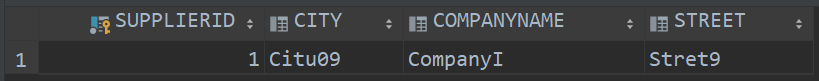
\includegraphics{images/point7/SelectSuppliers.png}
    \end{center}

    \subsubsection{Tabela Products}
    \begin{center}
        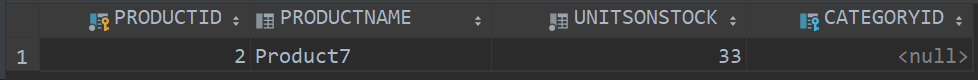
\includegraphics[scale=0.85]{images/point7/SelectProducts.png}
    \end{center}

    \subsubsection{Tabela Invoice}
    \begin{center}
        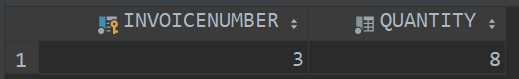
\includegraphics{images/point7/SelectInvoice.png}
    \end{center}

    \subsubsection{Tabela InvoiceProducts}
    \begin{center}
        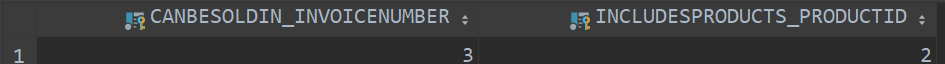
\includegraphics[scale=0.85]{images/point7/SelectInvoiceProducts.png}
    \end{center}

    \newpage

    \subsection{Kod DDL}
    \lstinputlisting{source_code_and_ddl/point7/DDL.sql}

    \newpage



    \section{IX. JPA. Zadanie z punktu VI z wykorzystaniem JPA}

    \subsection{Kod klasy Main - klasa nie wykorzystująca JPA}
    \lstinputlisting[firstline=2]{source_code_and_ddl/point9/Main.java}

    \newpage

    \subsection{Kod klasy MainJpa - klasa wykorzystująca JPA}
    \lstinputlisting[firstline=2]{source_code_and_ddl/point9/MainJpa.java}

    \newpage

    \subsection{Pobranie informacji o firmie, produkcie i kategorii}
    \begin{center}
        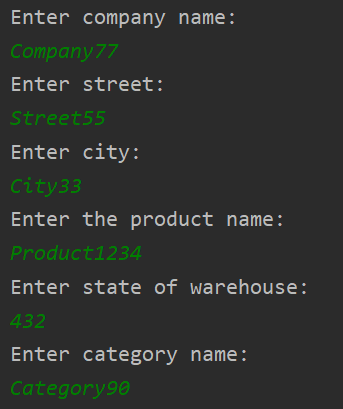
\includegraphics[scale=1.3]{images/point9/addCompanyProductAndCategory.png}
    \end{center}

    \subsection{Zapytania wykonane przez Hibernate}
    \begin{center}
        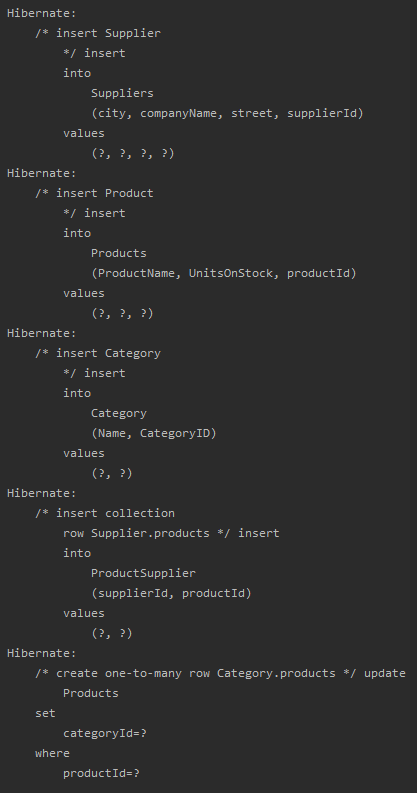
\includegraphics[scale=1.3]{images/point9/hibernateQueries.png}
    \end{center}

    \newpage


    \subsection{Wyniki SELECT * z poszczególnych tabel}

    \subsubsection{Tabela Suppliers}
    \begin{center}
        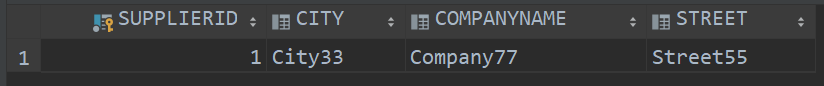
\includegraphics{images/point9/SelectSuppliers.png}
    \end{center}

    \subsubsection{Tabela Products}
    \begin{center}
        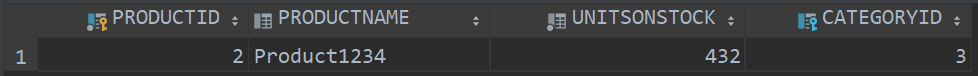
\includegraphics[scale=0.85]{images/point9/SelectProducts.png}
    \end{center}

    \subsubsection{Tabela ProductsSupplier}
    \begin{center}
        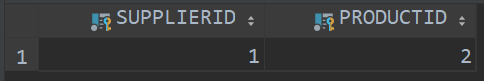
\includegraphics{images/point9/SelectProductsSupplier.png}
    \end{center}

    \subsubsection{Tabela Categories}
    \begin{center}
        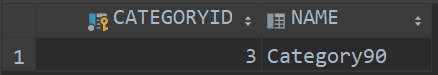
\includegraphics[scale=0.85]{images/point9/SelectCategories.png}
    \end{center}

    \newpage

    \subsection{Kod DDL}
    \lstinputlisting{source_code_and_ddl/point9/DDL.sql}

    \newpage


    \section{X. Cascade}

    \subsection{Kod klasy Invoice}
    \lstinputlisting[firstline=2]{source_code_and_ddl/point10/Invoice.java}

    \subsection{Kod klasy Product}
    \lstinputlisting[firstline=2]{source_code_and_ddl/point10/Product.java}



    \section{XI. Embedded class}

    \subsection{Pobranie informacji o firmie, produkcie i kategorii}
    \begin{center}
        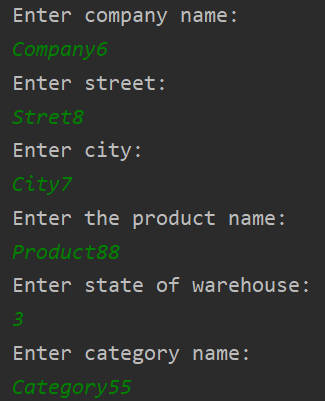
\includegraphics[scale=1.3]{images/point11/addCompanyProductAndCategory.png}
    \end{center}

    \subsection{Zapytania wykonane przez Hibernate}
    \begin{center}
        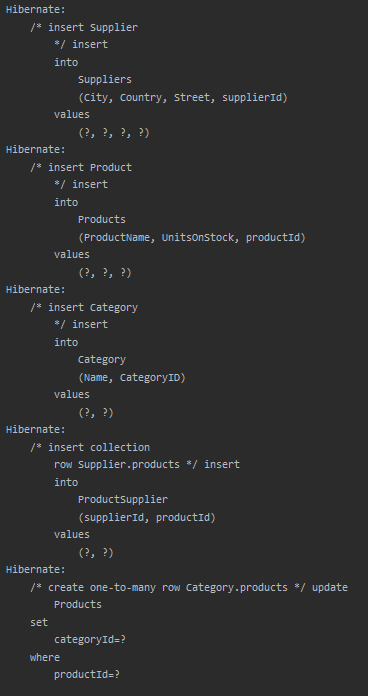
\includegraphics[scale=1.3]{images/point11/hibernateQueries.png}
    \end{center}

    \subsection{Kod klasy Address}
    \lstinputlisting[firstline=2]{source_code_and_ddl/point11/Address.java}

    \subsection{Kod klasy Supplier}
    \lstinputlisting[firstline=2]{source_code_and_ddl/point11/Supplier.java}

    \subsection{Wyniki SELECT * z poszczególnych tabel}

    \subsubsection{Tabela Suppliers}
    \begin{center}
        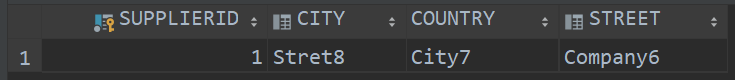
\includegraphics{images/point11/SelectSuppliers.png}
    \end{center}

    \subsubsection{Tabela Products}
    \begin{center}
        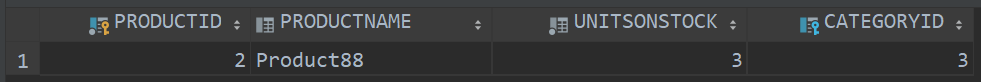
\includegraphics[scale=0.85]{images/point11/SelectProducts.png}
    \end{center}

    \subsubsection{Tabela ProductsSupplier}
    \begin{center}
        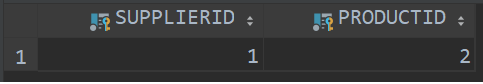
\includegraphics{images/point11/SelectProductsSupplier.png}
    \end{center}

    \subsubsection{Tabela Categories}
    \begin{center}
        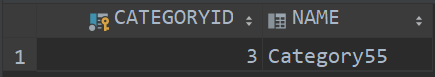
\includegraphics[scale=0.85]{images/point11/SelectCategories.png}
    \end{center}

    \newpage

    \subsection{Kod DDL}
    \lstinputlisting{source_code_and_ddl/point9/DDL.sql}

    \newpage



    \section{XII. Inheritance}

    \subsection{Kod klasy Company - Table Per Class}
    \lstinputlisting[firstline=2]{source_code_and_ddl/point12/Company.java}

    \newpage

    \subsection{Kod klasy Company - Table Joined}
    \lstinputlisting[firstline=2]{source_code_and_ddl/point12/Company2.java}

    \newpage

    \subsection{Kod klasy Company - Single table}
    \lstinputlisting[firstline=2]{source_code_and_ddl/point12/Company3.java}

    \newpage

    \subsection{Kod klasy Customer}
    \lstinputlisting[firstline=2]{source_code_and_ddl/point12/Customer.java}

    \newpage

    \subsection{Kod klasy Supplier}
    \lstinputlisting[firstline=2]{source_code_and_ddl/point12/Supplier.java}


    \newpage

    \section{Kod niektórych klas wykorzystanych w projekcie}

    \subsection{Kod klasy Creator - wykorzystywanej do pobierania informacji od użytkownika}
    \lstinputlisting[firstline=2]{source_code_and_ddl/classes_used/Creator.java}

    \newpage

    \subsection{Kod klasy DatabasePerformer - wykorzystywanej do wykonywania różnych operacji na bazie danych}
    \lstinputlisting[firstline=2]{source_code_and_ddl/classes_used/DatabasePerformer.java}

\end{document}
